\documentclass[11pt]{article}
\usepackage[margin=23mm]{geometry}
\usepackage{amsmath,amssymb,graphicx,booktabs,hyperref}
\newcommand{\issue}[2]{\subsection*{Comment #1. #2}}
\title{Response to the referee\\\large Hybrid Chiral Skin Correlated States in Monitored Quantum Circuits}
\date{Working draft for author review}
\begin{document}
\maketitle
Dear Referee,

Thank you for asking how interactions modify chiral skin modes and how an experiment could distinguish these changes. We address the eleven comments in report order. We evaluate occupations and quantum correlations using the normalized right state, consistent with conditional pure-state measurements. The dominant state denotes the right eigenstate with largest imaginary energy when isolated.

\issue{1}{Distinction from conventional many-body and Fock-space skin effects}
Our contribution concerns the joint real-space distribution of two fermions on a physical chiral boundary. Concentration in a subset of Fock configurations alone leaves their spatial support undetermined. We therefore compare the edge fraction, adjacent-cell pair probability and directional motion. On the $4\times4$ sample at $u=-1.5,\gamma=0.2$, raising $U$ from 0 to 1 increases the dominant-state edge fraction from 0.376 to 0.510 and the adjacent-pair probability from 0.215 to 0.715. For a Fock configuration $q$, let $b(q)=\sum_{\langle ij\rangle}N_i(q)N_j(q)$ in terms of cell occupations. A hop to $q'$ then changes the interaction energy by $U[b(q')-b(q)]$. Only hops changing the number of occupied neighbour pairs acquire this detuning. This qualifies the energy-isolation argument in the Mechanism subsection. The trivial-parent control in Comment 11 also shows pair enhancement. We attribute the hybrid character to the coexistence of directional edge motion and interaction-induced correlations.

\issue{2}{Localization and correlations versus interaction strength}
Using the gain edge as $y=0$, we measure the transverse width $w_y=[\sum_{xy} y^2\langle N_{xy}\rangle/2]^{1/2}$. For the same dominant state, at $U=0,1,2$ we obtain $w_y=1.947,1.342,0.713$ cells. The Frobenius norm of the off-diagonal connected density correlator is 0.118, 0.309 and 0.406, respectively. The adjacent-pair probability increases particularly rapidly between $U=0.5$ and $0.75$ (0.197 to 0.673). Reselecting the dominant state at each point allows a change of spectral branch. These numbers identify a finite-sample crossover interval. Assigning an exponential localization length would require a resolved exponential tail, and assigning a critical interaction would require size convergence. The squared overlap of the normalized $t=10$ state with the dominant state at $U=1$ is only 0.495, so we report these two states separately.

\issue{3}{Topological invariant or bulk-boundary correspondence}
The dissipative chiral edge channel explains the single-particle accumulation [1]. The correspondence between Hermitian bulk topology and dissipative boundary topology holds under specified symmetry, boundary and gap conditions [2,3]. These results establish the single-particle basis of our mechanism. We agree that our evidence does not establish protection of the interacting eigenvector or its entanglement. We propose to restrict the protection claim to the applicable parent boundary modes and describe the extra pair correlation as interaction induced. A candidate diagnostic for a stronger claim is the fixed-sector winding [4],
\[
W_2(E_*)=(2\pi i)^{-1}\int_0^{2\pi}d\phi\,\partial_\phi\log\det[H_2(\phi)-E_*].
\]
This requires twisting the periodic direction of a strip and verifying a point gap throughout flux insertion. Even a winding of the full two-particle spectrum would require a separate correspondence to the particular open-boundary state of interest. Such a correspondence remains open here.

\issue{4}{Origin, quantification and robustness of chirality}
We prepare two adjacent B modes symmetrically about the centre of the gain edge and measure $X_e(t)=\sum_x(x-1.5)\langle N_{x,0}(t)\rangle/2$ on a $4\times4$ sample. Conjugating the Hermitian hopping reverses the parent chirality at fixed gain, initial state and interaction. At $U=1,\gamma=0.2,t=2$ the signed moments for the two orientations are $-0.04339,+0.04339$ cells. The trivial parent ($u=-2.5$) also reverses direction but gives a magnitude of only 0.00150. Both magnitude and sign are relevant because the observable weights displacement by the population on the edge. The stationary disorder test below addresses localization. Directional robustness over a disorder ensemble remains unquantified.

\issue{5}{Disorder, hopping variations and broken symmetry}
We additionally diagonalized the two-particle $3\times3$ model at $u=-1.5,\gamma=0.2,U=1$. Real onsite shifts are independent and uniform in $[-0.1,0.1]$. In a separate ensemble each physical hopping receives a real uniform factor in $[0.9,1.1]$, shared by the conjugate hopping and all spectator configurations. A separate local potential of 0.1 on the first A mode breaks A/B exchange. Entries for the random ensembles are means and sample standard deviations for 12 realizations each.
\begin{center}\begin{tabular}{lcc}\toprule
Perturbation & Edge fraction & Adjacent-pair probability\\\midrule
Clean &0.451&0.099\\
Onsite disorder &$0.479\pm0.040$&$0.472\pm0.305$\\
Random hopping &$0.454\pm0.016$&$0.381\pm0.282$\\
Local A potential &0.460&0.078\\\bottomrule
\end{tabular}\end{center}
The edge fraction is comparatively stable at these strengths. Pair probabilities vary substantially across samples, allowing for reselection of the dominant state. The data give neither a universal disorder threshold nor evidence for protected pair correlations.

\issue{6}{Quantitative quantum entanglement}
For a normalized pure state $\sum_{i<j} A_{ij}c_i^\dagger c_j^\dagger|0\rangle$, extend $A$ antisymmetrically. The squared singular values of $A$ give the natural occupations $n_a$, which sum to two. The one-body linear-entropy diagnostic $D=\sum_a n_a(1-n_a)/2$ vanishes precisely for a single Slater determinant. It measures correlations beyond antisymmetrization. At $L=4$ we find $D<10^{-12}$ for the dominant state at $U=0$ and $D=0.663$ at $U=1$. For the $t=10$ state the values are below $10^{-12}$ and 0.623. This supplies quantum-state information beyond the density correlations. The entropy of a spatial cut measures entanglement between two mode sets and can already be finite at $U=0$.

\issue{7}{Particle number, dimension and geometry}
To compare particle numbers, we divide the edge occupation by $n$ and the expected number of adjacent-cell particle pairs by $\binom n2$. On the clean $3\times3$ sample of Comment 5, the dominant-state edge fractions for $n=2,3$ are 0.451 and 0.685. The corresponding adjacent-pair fractions are 0.099 and 0.497. Both increase in this example, where filling changes as well. The manuscript's three-excitation and 3D CSTI examples establish cases beyond the two-excitation 2D calculation. Generality across arbitrary filling, dimension or lattice geometry is still an open question.

\issue{8}{Computational scaling and the advantage of fixed excitation number}
With $M$ fermion modes, the sector dimension $d_n=\binom Mn$ grows as $M^n/n!$ at fixed $n$ and exponentially at fixed nonzero filling below unity. For $M=32,n=2$ we used $d_n=496$. One dense complex-double Hamiltonian occupies $16d_n^2$ bytes (3.75 MiB), excluding eigenvectors and workspace. Dense full diagonalization costs order $d_n^3$ operations. A sparse solver can target selected eigenpairs. The practical circuit advantage is programmable conditional evolution and access to site-resolved readout. These comparisons do not establish an end-to-end speedup.

\issue{9}{Post-selection probability and resources}
For the gain implementation the accepted auxiliary outcome acts as $K_i=\mathrm{diag}(e^{-\gamma\delta t},1)$. For $m$ monitored modes, the successful layer in our ideal split-step benchmark is $K e^{-iH_0\delta t}$ with $K=\exp[\gamma\delta t(N_e-m)]$. The cumulative success probability is the squared norm of the unnormalized layer product applied to the initial state. For $n\le m$ the minimum and maximum singular values bound it by
\[
 e^{-2\gamma mT}\le P_{\rm succ}\le e^{-2\gamma(m-n)T}.
\]
The $2\times4$ circuit uses 16 system qubits and one reusable auxiliary qubit, with $m=4,n=2$. At $T=4,\gamma=0.2,\delta t=0.05$ we obtain $P_{\rm succ}=0.01403$, with 80 layers and 320 local acceptance checks. Collecting 1,000 retained samples takes approximately 71,300 initial runs on average. Native gate depth depends on connectivity and compilation. These estimates quantify ideal overhead with an exact Hermitian substep.

\issue{10}{Finite-step corrections, random layers and anti-PT symmetry}
At fixed $T=4$, the conditional-state infidelities relative to exact evolution are $1.36\times10^{-3},3.41\times10^{-4},8.53\times10^{-5},2.14\times10^{-5}$ for $\delta t=0.4,0.2,0.1,0.05$. The local commutator error of the first-order split is order $\delta t^2$; first-order global amplitude error is consistent with the observed quadratic infidelity. Decomposing $H_0$ into native gates introduces additional errors. For independent Bernoulli measurement choices at one site, the measured layer fraction has variance $p(1-p)/N$. This accounts for the statistical scale of the measurement schedule but does not by itself give the error in a normalized conditioned state. Our benchmark uses $p=1$. In the manuscript convention the even interaction gives $\mathcal{PT}H(U)(\mathcal{PT})^{-1}=-H(-U)$. Hence pairing of the spectrum within one fixed $U$ need not persist. The correlated state at nonzero $U$ already occurs outside the single-particle anti-PT constraint. The local perturbation in Comment 5 supplies a further test.

\issue{11}{Experimental signature and sensitivity to noise}
Accepted occupation strings give both site densities and adjacent-pair counts. An experimental comparison can combine the $U=0,1$ pair probabilities with the signed edge-moment test in Comment 4. At $L=4,t=10$ the ideal adjacent-pair probabilities increase from 0.178 to 0.595 for the topological parent and from 0.155 to 0.694 for the trivial parent. Pair enhancement alone is therefore ambiguous. For 1,000 independent retained shots per interaction the predicted standard error of the first difference is $\sqrt{[0.178(1-0.178)+0.595(1-0.595)]/1000}=0.020$. This conditional estimate concerns a different size and time from the resource example in Comment 9. If $P$ is the true acceptance probability, $a$ the sequence-level efficiency conditional on success and $b$ the false acceptance probability conditional on failure, the contamination fraction is $b(1-P)/[aP+b(1-P)]$. Readout errors can thus have a disproportionately large effect at small $P$. Quantitative tolerances to imperfect gates and correlated readout errors remain to be determined for a specified noise model.

\begin{figure}[ht]\centering
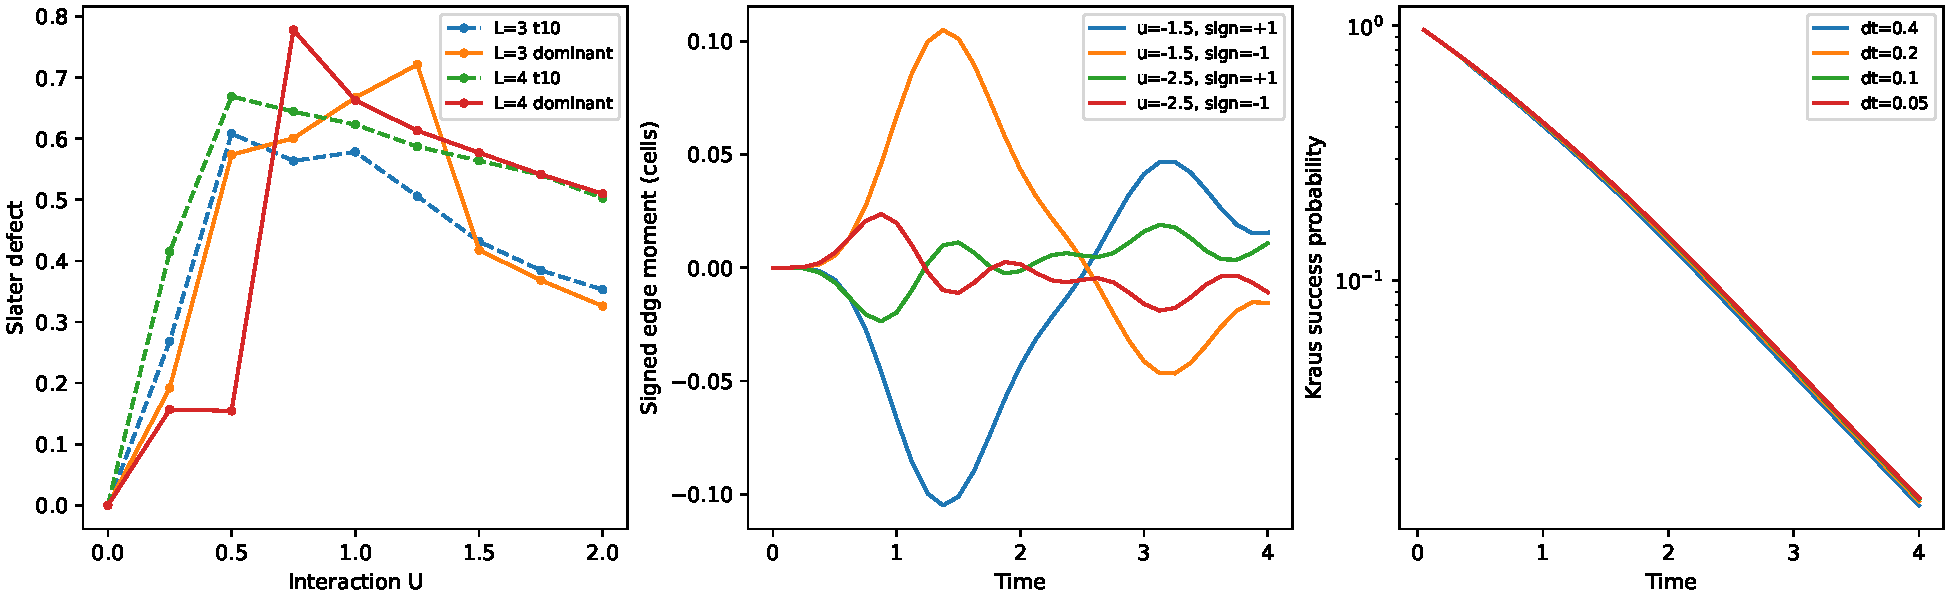
\includegraphics[width=\linewidth]{../code/results/reviewer_followup/followup.pdf}
\caption{Left: departure from a single Slater determinant for dominant and finite-time states. Centre: signed edge moment for opposite hopping orientations. Right: cumulative ideal acceptance in the two-particle split-step circuit.}
\end{figure}

\paragraph{References}
[1] X.-R. Ma et al., \emph{Chiral Skin Effect}, arXiv:2304.01422.
[2] F. Schindler et al., \emph{Hermitian Bulk -- Non-Hermitian Boundary Correspondence}, arXiv:2304.03742.
[3] D. Nakamura et al., \emph{Universal platform of point-gap topological phases from topological materials}, arXiv:2304.08110.
[4] K. Kawabata, K. Shiozaki and S. Ryu, \emph{Many-body topology of non-Hermitian systems}, Phys. Rev. B 105, 165137 (2022).
\end{document}
